\documentclass[10pt,a4paper,twocolumn,twoside]{article}
\usepackage[utf8]{inputenc}
\usepackage[catalan]{babel}
\usepackage{multicol}
\usepackage{graphicx}
\usepackage{fancyhdr}
\usepackage{times}
\usepackage{titlesec}
\usepackage{multirow}
\usepackage{lettrine}
\usepackage[top=2cm, bottom=1.5cm, left=2cm, right=2cm]{geometry}
\usepackage[figurename=Fig.,tablename=TAULA]{caption}
\captionsetup[table]{textfont=sc}

\author{\LARGE\sffamily Christian Espinosa Reboredo}
\title{\Huge{\sffamily Recognition of cognitive states from EEG data}}
\date{}

\newcommand\blfootnote[1]{%
  \begingroup
  \renewcommand\thefootnote{}\footnote{#1}%
  \addtocounter{footnote}{-1}%
  \endgroup
}

%
%\large\bfseries\sffamily
\titleformat{\section}
{\large\sffamily\scshape\bfseries}
{\textbf{\thesection}}{1em}{}

\begin{document}

\fancyhead[LO]{\scriptsize AUTOR: TÍTOL DEL TREBALL}
\fancyhead[RO]{\thepage}
\fancyhead[LE]{\thepage}
\fancyhead[RE]{\scriptsize EE/UAB TFG INFORMÀTICA: TÍTOL (ABREUJAT SI ÉS MOLT LLARG)}

\fancyfoot[CO,CE]{}

\fancypagestyle{primerapagina}
{
   \fancyhf{}
   \fancyhead[L]{\scriptsize TFG EN ENGINYERIA INFORMÀTICA, ESCOLA D'ENGINYERIA (EE), UNIVERSITAT AUTÒNOMA DE BARCELONA (UAB)}
   \fancyfoot[C]{\scriptsize ``Mes'' de 20xx, Escola d'Enginyeria (UAB)}
}

%\lhead{\thepage}
%\chead{}
%\rhead{\tiny EE/UAB TFG INFORMÀTICA: TÍTOL (ABREUJAT SI ÉS MOLT LLARG)}
%\lhead{ EE/UAB \thepage}
%\lfoot{}
%\cfoot{\tiny{February 2015, Escola d'Enginyeria (UAB)}}
%\rfoot{}
\renewcommand{\headrulewidth}{0pt}
\renewcommand{\footrulewidth}{0pt}
\pagestyle{fancy}

%\thispagestyle{myheadings}
\twocolumn[\begin{@twocolumnfalse}

%\vspace*{-1cm}{\scriptsize TFG EN ENGINYERIA INFORMÀTICA, ESCOLA D'ENGINYERIA (EE), UNIVERSITAT AUTÒNOMA DE BARCELONA (UAB)}

\maketitle

\thispagestyle{primerapagina}
%\twocolumn[\begin{@twocolumnfalse}
%\maketitle
%\begin{abstract}
\begin{center}
\parbox{0.915\textwidth}
{\sffamily
%\textbf{Resum--}

%\end{abstract}
%\bigskip
%\begin{abstract}
%\bigskip
%\\
\textbf{Abstract--}An electroencephalogram (EEG) is a test that detects electrical activity of the brain. Since 
1924 this procedure has been done countless times to obtain brain activity. This paper tries to go a step further 
to understand electroencephalography better using deep learning algorithms. The data used in this paper is a public 
dataset CHB-MIT of recordings of paediatric subjects with intractable seizures. Different methods of data management 
are done and documented to make the most of the algorithms used. The objective is to train an algorithm to acknowledge 
when the subject is having a seizure.
\\
\\
\textbf{Keywords-- }electroencephalogram, deep learning, brain activity, classification, EEG analysis\\
}

\bigskip

{\vrule depth 0pt height 0.5pt width 4cm\hspace{7.5pt}%
\raisebox{-3.5pt}{\fontfamily{pzd}\fontencoding{U}\fontseries{m}\fontshape{n}\fontsize{11}{12}\selectfont\char70}%
\hspace{7.5pt}\vrule depth 0pt height 0.5pt width 4cm\relax}

\end{center}

\bigskip
%\end{abstract}
\end{@twocolumnfalse}]

\blfootnote{$\bullet$ E-mail de contacte: christian.espinosar@uab.cat}
\blfootnote{$\bullet$ Menció realitzada: Computació }
\blfootnote{$\bullet$ Treball tutoritzat per: Aura Hernández Sabaté (Ciencies de la Computació)}
\blfootnote{$\bullet$ Curs 2021/22}

\section{Introduction}

\lettrine[lines=3]{A}{n} epileptic seizure is a period of symptoms due to abnormally excessive or synchronous 
neuronal activity in the brain. This can cause different effects like uncontrolled shaking movements involving much 
of the body, parts of the body or subtle momentary loss of awareness. In order to understand this issue, it is 
important to understand how neurons work and interact with each other to conserve what we call consciousness 
represented as brain activity and brainwaves. 
\\
To further understand we first need to study a single neuron. Neural oscillations are rhythmic or repetitive patterns 
of neural activity in the central nervous system which can be driven by mechanisms within individual neurons or by 
interactions. Since 1824 neural oscillations have been observed, fifty years later intrinsic oscillatory behaviour 
was encountered in vertebrate neurons, but the purpose of these is yet to be fully understood.
\\
In order to understand better brain activity this paper tries to dig deeper using new technology like deep learning 
to try to understand what humans are incapable of doing. First of all, it will be needed an inside view on how the 
brain works to have a hint on how to extract or intercept information from the neurons to process externally in a 
computer as well as a view on how deep learning algorithm’s function and get results from data, because it’s the 
best way to process and get the most out of it. Afterwards an insight of previous papers is given to set a view point 
on how research has been made up until this point. A well-known database (CHB-MIT) is introduced of encephalograms 
collected from 23 subject with interactable seizures that has been used in previous research.
\\
Once everything is acknowledged objectives of this paper are settled for further research on this issue. First of all, 
data planning and different treatment procedures are important to see how algorithms behave giving better or worse 
results, as well as which algorithm architectures are better to process EEG data. Finally, once all the research is 
done the classifier is to be expected to classify moments where seizures occur on the patients in a given moment.
\\

\section{Brain structure}
To further understand how the brain proceses input readings from we first need to study a single neuron. 
\begin{itemize}
\item de 8 a 10 pàgines d’explicació del treball, agraïments i bibliografia.
\item 4 pàgines addicionals per incloure matèria d’apèndix.
\end{itemize}

L'organització en seccions dependrà de cada treball, però de manera genèrica podem esperar:

\begin{itemize}
\item Secció d’introducció on s’explica el context del treball i les motivacions i es plantegen els objectius. També s’explica breument l’organització de la resta del document.
\item Una sèrie de seccions que dependran del treball particular.
\item Una secció on es presenti el mètode d’avaluació dels resultats, els resultats en si mateixos, i una discussió/reflexió sobre aquests resultats.
\item Una secció de conclusió del treball, apuntant també les línies de continuació.
\item Uns petits agraïments, si s’escau.
\item La bibliografia.
\item Una secció a mode d’apèndix, si s’escau.
\end{itemize}

\section{Exemple de Secció}

Això és un exemple de secció que conté dues subseccions (\ref{subsec-exemple1} i \ref{subsec-exemple2}) i una figura (\ref{fig-exemple}).

\subsection{Exemple de subsecció}
\label{subsec-exemple1}

.... ..  .... .. .... ... ..... ... ..... ... ... ..... .... .


% Per a fer que la figura ocupi les dues columnes utilitzeu "figure*" per comptes de "figure"
\begin{figure}[!h]
\centering
	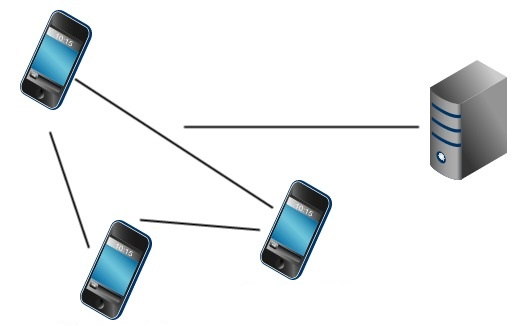
\includegraphics[width=0.4\textwidth]{img/adhoc_dtn}
	\caption{Exemple de figura}
	\label{fig-exemple}
\end{figure}

\subsection{Un altre exemple de subsecció}
\label{subsec-exemple2}

La taula \ref{tab:senzilla} és un exemple de taula senzilla. En canvi, la taula \ref{tab:taula2} és més completa.

Hi ha moltes referències \textit{on-line} de \LaTeX, com \cite{latex}.

% Utilitzeu el begin table només en cas de vole taules flotants. Si les voleu al lloc, tabular directament.
\begin{table}
\caption{Taula d'exemple}
\label{tab:senzilla}
\begin{center}
\begin{tabular}{|c|c|}
\hline
One & Two\\
\hline
Three & Four\\
\hline
\end{tabular}
\end{center}
\end{table}



\begin{table}
\caption{Taula més completa}
\label{tab:taula2}

\begin{center}
\begin{tabular}{ |l|l|l| }
\hline
\multicolumn{3}{ |c| }{Team sheet} \\
\hline
Goalkeeper & GK & Paul Robinson \\ \hline
\multirow{4}{*}{Defenders} & LB & Lucus Radebe \\
 & DC & Michael Duburry \\
 & DC & Dominic Matteo \\
 & RB & Didier Domi \\ \hline
\multirow{3}{*}{Midfielders} & MC & David Batty \\
 & MC & Eirik Bakke \\
 & MC & Jody Morris \\ \hline
Forward & FW & Jamie McMaster \\ \hline
\multirow{2}{*}{Strikers} & ST & Alan Smith \\
 & ST & Mark Viduka \\
\hline
\end{tabular}
\end{center}
\end{table}

\section{Conclusions}

.... ..  .... .. .... ... ..... ... ..... ... ... ..... .... .
.... ..  .... .. .... ... ..... ... ..... ... ... ..... .... .
.... ..  .... .. .... ... ..... ... ..... ... ... ..... .... .
.... ..  .... .. .... ... ..... ... ..... ... ... ..... .... .
.... ..  .... .. .... ... ..... ... ..... ... ... ..... .... .
.... ..  .... .. .... ... ..... ... ..... ... ... ..... .... .
.... ..  .... .. .... ... ..... ... ..... ... ... ..... .... .
.... ..  .... .. .... ... ..... ... ..... ... ... ..... .... .
.... ..  .... .. .... ... ..... ... ..... ... ... ..... .... .
.... ..  .... .. .... ... ..... ... ..... ... ... ..... .... .
.... ..  .... .. .... ... ..... ... ..... ... ... ..... .... .
.... ..  .... .. .... ... ..... ... ..... ... ... ..... .... .
.... ..  .... .. .... ... ..... ... ..... ... ... ..... .... .
.... ..  .... .. .... ... ..... ... ..... ... ... ..... .... .

\section*{Agraïments}

... ..  .... .. .... ... ..... ... ..... ... ... ..... .... .
.... ..  .... .. .... ... ..... ... ..... ... ... ..... .... .
.... ..  .... .. .... ... ..... ... ..... ... ... ..... .... .
.... ..  .... .. .... ... ..... ... ..... ... ... ..... .... .
.... ..  .... .. .... ... ..... ... ..... ... ... ..... .... .

\begin{thebibliography}{11}

\bibitem{neural_oscilation}
https://en.wikipedia.org/wiki/Neural\_oscillation

\bibitem{seizure}
https://en.wikipedia.org/wiki/Seizure

\bibitem{latex}
http://en.wikibooks.org/wiki/LaTeX

\bibitem{the}
http://www.acnweb.org/acta/2002\_18\_2\_104.pdf

\bibitem{other projects}
https://arxiv.org/pdf/1908.10432v1.pdf

\bibitem{dataset}
https://paperswithcode.com/dataset/chb-mit



\end{thebibliography}

\appendix

\section*{Apèndix}

\setcounter{section}{1}

\subsection{Secció d'Apèndix}


... ..  .... .. .... ... ..... ... ..... ... ... ..... .... .
.... ..  .... .. .... ... ..... ... ..... ... ... ..... .... .
.... ..  .... .. .... ... ..... ... ..... ... ... ..... .... .
.... ..  .... .. .... ... ..... ... ..... ... ... ..... .... .
.... ..  .... .. .... ... ..... ... ..... ... ... ..... .... .

\subsection{Secció d'Apèndix}


... ..  .... .. .... ... ..... ... ..... ... ... ..... .... .
.... ..  .... .. .... ... ..... ... ..... ... ... ..... .... .
.... ..  .... .. .... ... ..... ... ..... ... ... ..... .... .
.... ..  .... .. .... ... ..... ... ..... ... ... ..... .... .
.... ..  .... .. .... ... ..... ... ..... ... ... ..... .... .


\end{document}

